\chapter{Введение}

\section{Цель работы}

Получение навыков проектирования БД, знакомство с синтаксисом СУБД PostgreSQL, создание ER-диаграммы.

\section{Теоретическая информация}

Проектирование любой базы данных начинается с описания предметной области. Для переноса предметной области в концептуальную схему БД необходимо определить сущности и связи между ними для полного представления выбранной предметной области. Для визуализации процесса используются ER-диаграммы (сущность-связь), которые возможно преобразовать в операторы создания необходимого набора операторов для создания отношения и связей в БД. Существует множество прикладных программ, реализующих данный функционал без выгрузки в БД (Visio) и с поддержкой выгрузки в определенную версию БД.
В курсе лабораторных работ в качестве основной используется PostgreSQL, поэтому все действия необходимо производить в данной СУБД.

\chapter{Ход работы}


Для предметной области был выбран интернет-магазин цветов.

\begin{figure}[h!]
	\centering
	\caption{EER-диаграмма}
	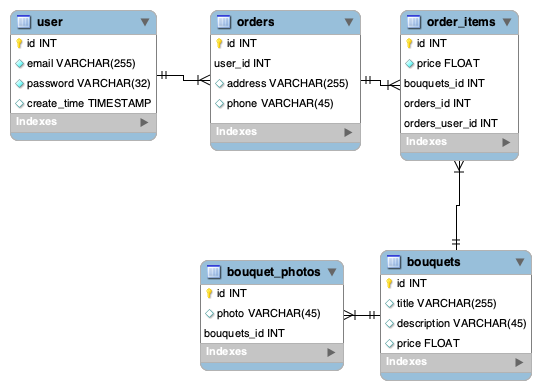
\includegraphics[width=.9\textwidth]{images/EER.png}
\end{figure}

\lstinputlisting{src/users.sql}

\lstinputlisting{src/bouquets.sql}

\lstinputlisting{src/bouquet_photos.sql}

\lstinputlisting{src/orders.sql}

\lstinputlisting{src/order_items.sql}

\lstinputlisting{src/mysql.in}
